\documentclass[11pt,a4paper]{article}
\usepackage[utf8]{inputenc}
\usepackage[T1]{fontenc}
\usepackage{lmodern}
\usepackage[french]{babel}
\usepackage[margin=2.3cm]{geometry}
\usepackage{amsmath,amssymb,mathtools}
\usepackage{bm}
\usepackage{graphicx}
\usepackage{booktabs}
\usepackage{enumitem}
\usepackage[dvipsnames]{xcolor}
\usepackage[most]{tcolorbox}
\usepackage{listings}
\usepackage{hyperref}
\hypersetup{colorlinks=true,linkcolor=NavyBlue}
\usepackage{fancyhdr}
\pagestyle{fancy}\fancyhf{}
\lhead{\small ECN-6025 -- Inférence et tests d'hypothèse}\rhead{\small Corrigé des exercices}\cfoot{\thepage}
\setlength{\headheight}{14pt}
\setlength{\parskip}{0.5em}\setlength{\parindent}{0pt}

\newcommand{\vy}{\mathbf{y}}\newcommand{\vX}{\mathbf{X}}\newcommand{\vZ}{\mathbf{Z}}\newcommand{\vb}{\mathbf{b}}
\newcommand{\vx}{\mathbf{x}}\newcommand{\ve}{\mathbf{e}}\newcommand{\vu}{\mathbf{u}}\newcommand{\vr}{\mathbf{r}}\newcommand{\R}{\mathbf{R}}
\newcommand{\vbeta}{\bm{\beta}}\newcommand{\vgamma}{\bm{\gamma}}\newcommand{\veps}{\bm{\epsilon}}
\newcommand{\I}{\mathbf{I}}\newcommand{\Pm}{\mathbf{P}}
\newcommand{\E}{\mathbb{E}}\newcommand{\Var}{\operatorname{Var}}\newcommand{\Cov}{\operatorname{Cov}}
\newcommand{\plim}{\operatorname{plim}}
\newcommand{\sumi}{\sum_{i=1}^{n}}

\newtcolorbox{idee}[1][]{colback=Cerulean!6,colframe=Cerulean!70!black,fonttitle=\bfseries,title={Idée de la démarche},#1}
\newtcolorbox{reponse}[1][]{colback=ForestGreen!6,colframe=ForestGreen!70!black,fonttitle=\bfseries,title={Réponse},#1}
\newtcolorbox{intuition}[1][]{colback=Goldenrod!8,colframe=Goldenrod!70!black,fonttitle=\bfseries,title={Intuition},#1}
\newtcolorbox{attention}[1][]{colback=BrickRed!5,colframe=BrickRed!75!black,fonttitle=\bfseries,title={Attention},#1}
\newtcolorbox{greene}[1][]{colback=gray!6,colframe=gray!55!black,fonttitle=\bfseries,title={Référence Greene},#1}

\lstset{basicstyle=\ttfamily\small,breaklines=true,frame=single,backgroundcolor=\color{gray!6},
  columns=fullflexible,keepspaces=true,showstringspaces=false,
  literate={é}{{\'e}}1 {è}{{\`e}}1 {à}{{\`a}}1 {ê}{{\^e}}1 {ç}{{\c{c}}}1 {É}{{\'E}}1}

\begin{document}

\begin{center}
{\LARGE\bfseries Inférence et tests d'hypothèse : corrigé}\\[6pt]
{\large Intervalles de confiance, tests $t$ et $F$, contraintes linéaires, Monte Carlo}\\[4pt]
{\small S'appuie sur W. H. Greene, \emph{Econometric Analysis} (ch. 4, 5, 8, 9 et 20)}
\end{center}

\begin{greene}
\begin{itemize}[nosep]
\item \textbf{Ch. 4} : loi des MCO sous normalité, $\vb\mid\vX\sim N(\vbeta,\sigma^2(\vX'\vX)^{-1})$ ; statistique $t$ et intervalles de confiance ; Monte Carlo.
\item \textbf{Ch. 5} : tests d'hypothèses linéaires $\R\vbeta=\vr$, statistique $F$ (version Wald et version « somme des carrés des résidus contrainte / non contrainte »), estimation sous contrainte, reparamétrisation.
\item \textbf{Ch. 9} : hétéroscédasticité et écarts-types robustes de White. \textbf{Ch. 8} : endogénéité, variables instrumentales et doubles moindres carrés.
\end{itemize}
\end{greene}

\textbf{Les deux formules de base} (Greene, ch. 4--5). Sous normalité des erreurs, avec $s^2=\ve'\ve/(n-K)$ :
\[
t=\frac{b_k-\beta_k^0}{\text{e.t.}(b_k)}\sim t(n-K),\qquad \text{e.t.}(b_k)=\sqrt{s^2\,[(\vX'\vX)^{-1}]_{kk}},
\]
\[
F=\frac{(\text{SCE}_r-\text{SCE}_u)/r}{\text{SCE}_u/(n-K)}\sim F(r,\,n-K).
\]

\tableofcontents

% =====================================================================
\section{Exercice 1 : intervalle de confiance et test $t$}
% =====================================================================

Données : $b_k=5$, \ $\hat\sigma=s=1$ (erreur-type de la régression), \ $[(\vX'\vX)^{-1}]_{kk}=0{,}04$, \ $\alpha=0{,}05$.

\begin{attention}
L'énoncé ne précise ni l'hypothèse nulle ni la taille de l'échantillon. On teste l'hypothèse usuelle $H_0:\beta_k=0$ contre $H_1:\beta_k\neq0$, et on utilise la valeur critique 1,96 (grand échantillon). Avec $n-K$ degrés de liberté connus, il faudrait $t_{0{,}975;\,n-K}$, un peu plus grand ; les conclusions ne changent pas ici.
\end{attention}

\subsection*{1. Intervalle de confiance à 95\,\%}

\textbf{Étape 1 : l'écart-type de $b_k$.} D'après la formule $\widehat{\Var}(\vb)=s^2(\vX'\vX)^{-1}$ :
\[
\text{e.t.}(b_k)=\sqrt{s^2\,[(\vX'\vX)^{-1}]_{kk}}=\sqrt{1^2\times0{,}04}=0{,}2 .
\]
\textbf{Étape 2 : la formule de l'IC.} Comme $\frac{b_k-\beta_k}{\text{e.t.}(b_k)}$ suit une loi de Student (environ $N(0,1)$ en grand échantillon), $P\big(-1{,}96\le\frac{b_k-\beta_k}{\text{e.t.}}\le1{,}96\big)=0{,}95$, d'où
\[
\text{IC}_{95\%}(\beta_k)=b_k\pm1{,}96\times\text{e.t.}(b_k)=5\pm1{,}96\times0{,}2=5\pm0{,}392 .
\]

\begin{reponse}
$\text{IC}_{95\%}(\beta_k)=[4{,}608\ ;\ 5{,}392]$. Interprétation : si l'on répétait l'échantillonnage un grand nombre de fois, 95\,\% des intervalles construits ainsi contiendraient la vraie valeur $\beta_k$.
\end{reponse}

\subsection*{2. Statistique $t$}
\[
t=\frac{b_k-0}{\text{e.t.}(b_k)}=\frac{5}{0{,}2}=25 .
\]

\subsection*{3. Décision au seuil de 5\,\%}
\begin{reponse}
$|t|=25>1{,}96$ : on \textbf{rejette} $H_0:\beta_k=0$. C'est cohérent avec l'IC, qui ne contient pas 0 (dualité IC--test).
\end{reponse}

\subsection*{4. $p$-value}
\begin{reponse}
$p=2\,P(|T|>25)\approx0$ (de l'ordre de $10^{-137}$ avec la loi normale). \textbf{Interprétation} : si $\beta_k$ était vraiment nul, la probabilité d'obtenir une estimation aussi éloignée de 0 que 5 (soit 25 écarts-types) serait pratiquement nulle. Comme $p<0{,}05$, on rejette $H_0$ : $\beta_k$ est statistiquement significatif.
\end{reponse}

% =====================================================================
\section{Exercice 2 : test d'une combinaison linéaire $\beta_1+\beta_2=2$}
% =====================================================================

Données : $\hat\beta_1=1{,}2$ ; $\hat\beta_2=0{,}8$ ; $\Var(\hat\beta_1)=0{,}04$ ; $\Var(\hat\beta_2)=0{,}03$ ; $\Cov(\hat\beta_1,\hat\beta_2)=0{,}01$ ; $n-K=12$ ; valeur critique $2{,}18$.

\subsection*{1. Écart-type de $\hat\beta_1+\hat\beta_2$}

\begin{idee}
Variance d'une somme de deux variables aléatoires corrélées : $\Var(A+B)=\Var(A)+\Var(B)+2\Cov(A,B)$. \textbf{Ne pas oublier la covariance} : $\hat\beta_1$ et $\hat\beta_2$ sont estimés sur les mêmes données.
\end{idee}
\[
\Var(\hat\beta_1+\hat\beta_2)=0{,}04+0{,}03+2\times0{,}01=0{,}09
\qquad\Longrightarrow\qquad
\text{e.t.}(\hat\beta_1+\hat\beta_2)=\sqrt{0{,}09}=0{,}3 .
\]
(En écriture matricielle : $\R=(0,1,1,0)$, $\Var(\R\vb)=\R\,\widehat{\Var}(\vb)\,\R'$, Greene ch. 5.)

\subsection*{2. Hypothèse nulle pour $\gamma$}
On définit le paramètre $\gamma=\beta_1+\beta_2-2$ (l'énoncé écrit $\hat\beta$ : l'hypothèse porte sur les vrais paramètres, son estimateur est $\hat\gamma=\hat\beta_1+\hat\beta_2-2$).
\[
H_0:\gamma=0\qquad\text{contre}\qquad H_1:\gamma\neq0 .
\]

\subsection*{3. Le test}
\[
\hat\gamma=1{,}2+0{,}8-2=0,\qquad \text{e.t.}(\hat\gamma)=\text{e.t.}(\hat\beta_1+\hat\beta_2)=0{,}3,
\]
(soustraire la constante 2 ne change pas la variance), d'où
\[
t=\frac{\hat\gamma}{\text{e.t.}(\hat\gamma)}=\frac{0}{0{,}3}=0 .
\]

\begin{reponse}
$|t|=0<2{,}18=t_{0{,}975;\,12}$ : on \textbf{ne rejette pas} $H_0$. Les estimations vérifient exactement la contrainte ($\hat\beta_1+\hat\beta_2=2$) : les données sont parfaitement compatibles avec $\beta_1+\beta_2=2$ ($p$-value $=1$).

\textbf{Version par reparamétrisation} (Greene, ch. 5) : avec $\beta_1=\gamma+2-\beta_2$, le modèle devient
$y_i-2x_{1i}=\beta_0+\gamma\,x_{1i}+\beta_2(x_{2i}-x_{1i})+\beta_3x_{3i}+\epsilon_i$ ; le $t$ du coefficient de $x_{1i}$ est exactement celui calculé ci-dessus.
\end{reponse}

% =====================================================================
\section{Exercice 3 : transformer les contraintes en restrictions nulles}
% =====================================================================

\begin{idee}
Généraliser la reparamétrisation de l'exercice 2 : définir de nouveaux paramètres $\vgamma_1=\R\vbeta-\vr$, de sorte que la contrainte devienne $\vgamma_1=\mathbf 0$ (contrainte d'exclusion), puis réécrire le modèle en fonction de $\vgamma_1$.
\end{idee}

\textbf{Étape 1 : partitionner.} $\R$ est $r\times k$ de rang $r$ (contraintes non redondantes). Quitte à réordonner les colonnes de $\vX$, on écrit
\[
\R=[\R_1\ \ \R_2],\qquad \vbeta=\begin{pmatrix}\vbeta_1\\\vbeta_2\end{pmatrix},\qquad \vX=[\vX_1\ \ \vX_2],
\]
avec $\R_1$ de dimension $r\times r$ \textbf{inversible} et $\vbeta_1$ de dimension $r\times1$.

\textbf{Étape 2 : nouveaux paramètres.}
\[
\vgamma_1=\R_1\vbeta_1+\R_2\vbeta_2-\vr=\R\vbeta-\vr\quad(r\times1),\qquad \vgamma_2=\vbeta_2 .
\]
La contrainte $\R\vbeta=\vr$ équivaut à $\vgamma_1=\mathbf 0$.

\textbf{Étape 3 : exprimer $\vbeta_1$ en fonction de $\vgamma_1$.}
\[
\vbeta_1=\R_1^{-1}\big(\vgamma_1+\vr-\R_2\vbeta_2\big).
\]

\textbf{Étape 4 : substituer dans le modèle.}
\[
\vy=\vX_1\vbeta_1+\vX_2\vbeta_2+\vu=\vX_1\R_1^{-1}\vgamma_1+\vX_1\R_1^{-1}\vr-\vX_1\R_1^{-1}\R_2\vbeta_2+\vX_2\vbeta_2+\vu .
\]
On regroupe :
\[
\boxed{\ \underbrace{\vy-\vX_1\R_1^{-1}\vr}_{\vy^*}=\underbrace{\vX_1\R_1^{-1}}_{\vZ_1}\vgamma_1+\underbrace{\big(\vX_2-\vX_1\R_1^{-1}\R_2\big)}_{\vZ_2}\vbeta_2+\vu\ }
\]

\begin{reponse}
Le modèle $\vy^*=\vZ_1\vgamma_1+\vZ_2\vbeta_2+\vu$ est le même modèle que l'original (même ajustement, mêmes résidus, car $[\vZ_1\ \vZ_2]$ est une transformation inversible de $[\vX_1\ \vX_2]$ ; voir le devoir 1, question 1(a)). Les $r$ restrictions $\R\vbeta=\vr$ y deviennent $r$ \textbf{restrictions d'exclusion} $\vgamma_1=\mathbf 0$ : on teste que les $r$ variables $\vZ_1$ peuvent être retirées (test $F$ sur $\vZ_1$, ou test $t$ si $r=1$).

\textbf{Vérification sur l'exercice 2} : $\R=(0,1,1,0)$, $\vr=2$, on prend $\R_1=1$ (coefficient de $\beta_1$), $\R_2=(0,1,0)$ pour $(\beta_0,\beta_2,\beta_3)$. Alors $\vy^*=\vy-2\vx_1$, $\vZ_1=\vx_1$, et $\vZ_2=[\bm\iota,\ \vx_2-\vx_1,\ \vx_3]$ : c'est exactement la reparamétrisation de l'exercice 2.
\end{reponse}

% =====================================================================
\section{Exercice 4 : Monte Carlo du biais des MCO selon $n$}
% =====================================================================

Modèle : $y=\beta_1+\beta_2x_1+u$, $u\sim NID(0,1)$, $\beta_1=1$, $\beta_2=0{,}8$.

\subsection*{Les étapes}
\begin{enumerate}[nosep]
\item Fixer la graine ; choisir $n=25$ et générer $x_1$ \textbf{une seule fois} (par ex. $N(0,1)$), gardé fixe.
\item Répéter $R$ fois ($R\ge100$ ; ici $R=1000$) : tirer $u\sim N(0,1)$, construire $y=1+0{,}8x_1+u$, estimer par MCO, sauvegarder $\hat\beta_1$ et $\hat\beta_2$.
\item Calculer les moyennes $\bar{\hat\beta}_1,\bar{\hat\beta}_2$ et les biais estimés $\bar{\hat\beta}_1-1$ et $\bar{\hat\beta}_2-0{,}8$.
\item Recommencer avec $n=50,100,200$.
\end{enumerate}

\begin{lstlisting}
* Stata : une taille d'échantillon (changer N pour 25, 50, 100, 200)
clear all
set seed 2024
local N = 25
set obs `N'
gen x1 = rnormal()
gen y = .
tempname sim
postfile `sim' b1 b2 using mc_n`N', replace
quietly forvalues r = 1/1000 {
    replace y = 1 + 0.8*x1 + rnormal()
    regress y x1
    post `sim' (_b[_cons]) (_b[x1])
}
postclose `sim'
use mc_n`N', clear
summarize b1 b2        // moyennes -> biais = moyenne - vraie valeur
\end{lstlisting}

\subsection*{Résultats (réplication en Python, $R=1000$)}
\begin{center}
\begin{tabular}{@{}rcccccc@{}}
\toprule
$n$ & moy.\ $\hat\beta_1$ & moy.\ $\hat\beta_2$ & biais $\hat\beta_1$ & biais $\hat\beta_2$ & é.-t.\ $\hat\beta_2$ & erreur MC sur le biais de $\hat\beta_2$ \\
\midrule
25 & 1,0039 & 0,8086 & $+0{,}0039$ & $+0{,}0086$ & 0,198 & 0,0063 \\
50 & 1,0023 & 0,7982 & $+0{,}0023$ & $-0{,}0018$ & 0,154 & 0,0049 \\
100 & 0,9986 & 0,8024 & $-0{,}0014$ & $+0{,}0024$ & 0,091 & 0,0029 \\
200 & 0,9994 & 0,7980 & $-0{,}0006$ & $-0{,}0020$ & 0,069 & 0,0022 \\
\bottomrule
\end{tabular}
\end{center}

\begin{figure}[h]
\centering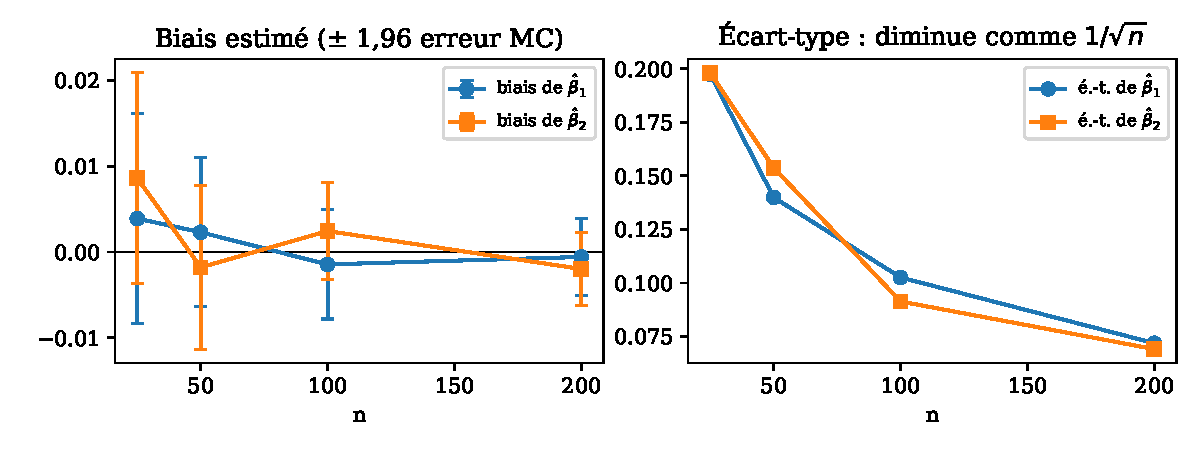
\includegraphics[width=0.92\textwidth]{figures/ex4_biais.pdf}
\caption{Gauche : biais estimés, toujours compatibles avec 0. Droite : la dispersion des estimateurs diminue avec $n$.}
\end{figure}

\begin{reponse}
\textbf{Le biais est nul pour toutes les tailles d'échantillon}, y compris $n=25$ : les biais estimés sont minuscules et du même ordre que l'erreur de simulation ($\text{é.-t.}/\sqrt R$), donc statistiquement indiscernables de 0. C'est attendu : sous $\E[\vu\mid\vX]=\mathbf 0$, les MCO sont \textbf{sans biais en échantillon fini} ($\E[\vb\mid\vX]=\vbeta$ pour tout $n$), le biais n'a donc pas à « diminuer ».

Ce qui change avec $n$, c'est la \textbf{précision} : l'écart-type de $\hat\beta_2$ diminue à peu près comme $1/\sqrt n$ (0,198 $\to$ 0,069 quand $n$ passe de 25 à 200, soit environ $\div\sqrt8\approx2{,}8$). Les biais estimés fluctuent donc de moins en moins autour de 0. C'est la convergence : $\Var(\vb)\to\mathbf 0$ et $\plim\vb=\vbeta$.
\end{reponse}

% =====================================================================
\section{Exercice 5 : estimer sous la contrainte $\beta_2+\beta_3=1$}
% =====================================================================

\textbf{Modèle contraint.} On remplace $\beta_3=1-\beta_2$ :
\[
y_t=\beta_1+\beta_2x_{t2}+(1-\beta_2)x_{t3}+u_t
\iff
\boxed{\ y_t-x_{t3}=\beta_1+\beta_2\,(x_{t2}-x_{t3})+u_t\ }
\]
On crée $y_t^*=y_t-x_{t3}$ et $z_t=x_{t2}-x_{t3}$, on régresse $y^*$ sur une constante et $z$. On obtient $\tilde\beta_1$, $\tilde\beta_2$, puis $\tilde\beta_3=1-\tilde\beta_2$ : la contrainte est respectée par construction. (C'est l'estimateur des moindres carrés contraints de Greene, ch. 5, obtenu ici par substitution.)

\textbf{Modèle non contraint reparamétré.} On pose $\gamma=\beta_2+\beta_3-1$, donc $\beta_3=\gamma+1-\beta_2$ :
\[
y_t=\beta_1+\beta_2x_{t2}+(\gamma+1-\beta_2)x_{t3}+u_t
\iff
\boxed{\ y_t-x_{t3}=\beta_1+\beta_2\,(x_{t2}-x_{t3})+\gamma\,x_{t3}+u_t\ }
\]

\begin{reponse}
\begin{itemize}[nosep]
\item \textbf{Contraint} : régresser $y_t-x_{t3}$ sur une constante et $(x_{t2}-x_{t3})$.
\item \textbf{Non contraint} : régresser $y_t-x_{t3}$ sur une constante, $(x_{t2}-x_{t3})$ \emph{et} $x_{t3}$. C'est le même modèle que l'original, et le coefficient de $x_{t3}$ est $\hat\gamma=\hat\beta_2+\hat\beta_3-1$.
\item Si les données respectent \textbf{exactement} la contrainte ($\hat\beta_2+\hat\beta_3=1$ dans la régression non contrainte), alors $\hat\gamma=0$ : le coefficient de $x_{t3}$ est nul. Le test $t$ de ce coefficient est le test de $H_0:\beta_2+\beta_3=1$.
\end{itemize}
\end{reponse}

% =====================================================================
\section{Exercice 6 : variable omise et hétéroscédasticité}
% =====================================================================

Vrai modèle : $y_i=\beta_0+\beta_1x_{1,i}+\beta_2x_{2,i}+\epsilon_i$, avec $x_{2,i}=\eta x_{1,i}+u_i$ ($\eta\neq0$), et $\Var(\epsilon_i\mid x_i)=\sigma_i^2$ non constante. On estime le modèle \textbf{court} $y_i=\beta_0+\beta_1x_{1,i}+\epsilon_i$.

\subsection*{1. Impact sur $\hat\beta_1$ et étude de Monte Carlo}

\textbf{Deux problèmes distincts se superposent.}
\begin{enumerate}
\item \textbf{L'omission de $x_2$ crée un biais} (si $\beta_2\neq0$), exactement comme à l'intra 2021 :
\[
\E[\hat\beta_1\mid x_1]=\beta_1+\beta_2\eta,\qquad \plim\hat\beta_1=\beta_1+\beta_2\eta .
\]
\item \textbf{L'hétéroscédasticité ne crée pas de biais}, mais elle change la variance (Greene, ch. 9). La vraie variance de la pente est
\[
\Var(\hat\beta_1\mid\vX)=\frac{\sum(x_{1,i}-\bar x_1)^2\,\sigma_i^2}{\big[\sum(x_{1,i}-\bar x_1)^2\big]^2}\neq\frac{\sigma^2}{\sum(x_{1,i}-\bar x_1)^2}\ \ \text{(formule MCO usuelle)}.
\]
L'écart-type affiché par défaut est donc \textbf{faux} (biaisé), et les MCO ne sont plus efficaces.
\end{enumerate}

\textbf{Étapes de la simulation.}
\begin{enumerate}[nosep]
\item Choisir $\beta_0,\beta_1,\beta_2,\eta$ (ex. $1,\ 1,\ 0{,}5,\ 0{,}5$), $n$, $R$, la graine, et une forme d'hétéroscédasticité, par ex. $\sigma_i^2=0{,}5+x_{1,i}^2$.
\item Générer une fois $x_1\sim N(0,1)$, $u\sim N(0,1)$, $x_2=\eta x_1+u$.
\item À chaque répétition : tirer $\epsilon_i=\sigma_i z_i$ avec $z_i\sim N(0,1)$ ; construire $y$ avec le vrai modèle ; régresser $y$ sur $(1,x_1)$ ; sauvegarder $\hat\beta_1$, l'écart-type classique et l'écart-type robuste de White.
\item Comparer : moyenne de $\hat\beta_1$ vs $\beta_1$ et $\beta_1+\beta_2\eta$ ; écart-type empirique des $\hat\beta_1$ (la vraie variabilité) vs moyenne des écarts-types classiques et robustes.
\end{enumerate}

\textbf{Ce qu'on obtient} (réplication Python, $R=2000$) :
\begin{center}
\begin{tabular}{@{}rccccc@{}}
\toprule
$n$ & moy.\ $\hat\beta_1$ & $\beta_1+\beta_2\hat\delta$ & é.-t.\ empirique & moy.\ é.-t.\ classique & moy.\ é.-t.\ White \\
\midrule
100 & 1,186 & 1,193 & 0,194 & 0,127 & 0,185 \\
1000 & 1,240 & 1,239 & 0,058 & 0,042 & 0,059 \\
\bottomrule
\end{tabular}
\end{center}
($\hat\delta$ : pente de la régression de $x_2$ sur $x_1$ dans l'échantillon simulé, proche de $\eta=0{,}5$.)

\begin{reponse}
\begin{itemize}[nosep]
\item \textbf{Biais} : $\hat\beta_1$ est centré sur $\beta_1+\beta_2\eta$, pas sur $\beta_1$ (variable omise). L'hétéroscédasticité n'y est pour rien et n'ajoute aucun biais.
\item \textbf{Variance} : la vraie variance de $\hat\beta_1$ suit la formule « sandwich » ci-dessus. La formule MCO usuelle la \textbf{sous-estime} ici (0,127 contre 0,194), parce que la variance des erreurs est plus forte là où $x_1$ est loin de sa moyenne. L'écart-type robuste de White, $\sqrt{[(\vX'\vX)^{-1}\vX'\hat{\bm\Sigma}\vX(\vX'\vX)^{-1}]_{22}}$, retrouve la bonne valeur. (Si la variance était au contraire plus forte près de la moyenne, la formule usuelle la surestimerait.)
\end{itemize}
\end{reponse}

\subsection*{2. Proportion de rejets de $H_0:\beta_2=0$ avec un test $t$ robuste}

Ce test se fait dans le modèle \textbf{complet} (qui contient $x_2$), avec des écarts-types de White.

\begin{reponse}
\begin{itemize}[nosep]
\item \textbf{Si la vraie valeur est $\beta_2=0$} ($H_0$ vraie) : on doit rejeter dans environ \textbf{5\,\%} des échantillons, soit le niveau $\alpha$ (erreur de type I). Le test robuste a la bonne taille \emph{asymptotiquement} ; en petit échantillon, il peut s'en écarter un peu. Simulation : 6,2\,\% pour $n=100$, 4,0\,\% pour $n=1000$.
\item \textbf{Si $\beta_2\neq0$} ($H_0$ fausse, comme dans l'exemple $\beta_2=0{,}5$) : la proportion de rejets est la \textbf{puissance} du test ; elle tend vers 100\,\% quand $n$ augmente. Simulation : 98,9\,\% pour $n=100$, 100\,\% pour $n=1000$.
\end{itemize}
Avec un test $t$ \emph{classique} (non robuste), la proportion de rejets sous $H_0$ ne serait en général pas égale à 5\,\% (l'écart-type est mal estimé) ; c'est pourquoi on utilise la version ajustée pour l'hétéroscédasticité.
\end{reponse}

% =====================================================================
\section{Exercice 7 : $x_i$ corrélé avec les erreurs}
% =====================================================================

\begin{attention}
L'énoncé écrit à la fois $\E[\epsilon\mid X]=0$ et « les $x_i$ sont corrélés avec les erreurs » : c'est contradictoire ($\E[\epsilon\mid X]=0$ implique $\Cov(x_i,\epsilon_i)=0$). On retient l'hypothèse qui fait l'objet de l'exercice : $\Cov(x_i,\epsilon_i)\neq0$ (endogénéité).
\end{attention}

\subsection*{1. Impact sur $\hat\beta$ et Monte Carlo}

\textbf{Biais attendu.} Comme à l'exercice 2 du document d'analyse asymptotique :
\[
\hat\beta=\beta+\frac{\frac1n\sum(x_i-\bar x)\epsilon_i}{\frac1n\sum(x_i-\bar x)^2}
\quad\Longrightarrow\quad
\plim\hat\beta=\beta+\frac{\Cov(x,\epsilon)}{\Var(x)}\neq\beta .
\]
$\hat\beta$ est \textbf{biaisé et non convergent} ; le biais a le signe de $\Cov(x,\epsilon)$ et ne disparaît pas quand $n$ augmente.

\textbf{Étapes de la simulation.}
\begin{enumerate}[nosep]
\item Choisir $\alpha$, $\beta$ (ex. $\alpha=0$, $\beta=1$), $n$, $R$, la graine.
\item À chaque répétition, générer \textbf{conjointement} $x$ et $\epsilon$ corrélés, par ex. $\epsilon_i\sim N(0,1)$, $z_i\sim N(0,1)$ et $x_i=\mu_x+z_i+0{,}5\,\epsilon_i$. (On ne peut pas garder $x$ fixe : il doit bouger avec $\epsilon$.) Ici $\Cov(x,\epsilon)=0{,}5$ et $\Var(x)=1{,}25$.
\item Construire $y_i=\alpha+\beta x_i+\epsilon_i$, estimer par MCO, sauvegarder $\hat\alpha$, $\hat\beta$ et le $t$ de $\hat\alpha$.
\item Comparer la moyenne des $\hat\beta$ à $\beta$ et à la valeur théorique $\beta+\Cov/\Var$ ; refaire pour plusieurs $n$.
\end{enumerate}

\begin{reponse}
Biais théorique : $\Cov(x,\epsilon)/\Var(x)=0{,}5/1{,}25=0{,}4$, donc $\hat\beta$ se concentre autour de $1{,}4$ au lieu de 1. Simulation ($R=2000$) : moyenne de $\hat\beta=1{,}400$ pour $n=100$ et $n=1000$ : le biais ne diminue pas avec $n$.
\end{reponse}

\subsection*{2. Proportion de rejets de $H_0:\alpha=0$}

\textbf{L'estimateur de la constante hérite du biais de la pente.} $\hat\alpha=\bar y-\hat\beta\bar x$, donc
\[
\plim\hat\alpha=\alpha+\beta\mu_x-(\plim\hat\beta)\mu_x=\alpha-\frac{\Cov(x,\epsilon)}{\Var(x)}\,\mu_x ,\qquad \mu_x=\E[x].
\]

\begin{reponse}
Supposons que la vraie valeur soit $\alpha=0$ ($H_0$ vraie).
\begin{itemize}[nosep]
\item \textbf{Si $\E[x]\neq0$} : $\hat\alpha$ converge vers $-0{,}4\,\mu_x\neq0$. Le test rejette $H_0$ (à tort) de plus en plus souvent, et la proportion de rejets tend vers \textbf{100\,\%} quand $n$ augmente. Simulation avec $\mu_x=2$ : 99,1\,\% ($n=100$) et 100\,\% ($n=1000$), au lieu de 5\,\%.
\item \textbf{Si $\E[x]=0$} : le biais de la pente ne contamine pas la constante à la limite, et la proportion de rejets reste proche de 5\,\% (simulation : 4,4\,\% et 5,8\,\%).
\end{itemize}
Leçon : avec des régresseurs endogènes, les tests ne contrôlent plus leur niveau. On ne rejette plus dans « $\alpha=5\,\%$ des cas sous $H_0$ » : l'inférence est invalide. La solution est d'utiliser des variables instrumentales (Greene, ch. 8 ; exercice 8).
\end{reponse}

% =====================================================================
\section{Exercice 8 : $\tilde\beta=(\vX'\Pm_z\vX)^{-1}\vX'\Pm_z\vy$ est sans biais}
% =====================================================================

C'est l'estimateur des \textbf{doubles moindres carrés} (Greene, ch. 8). Hypothèses : $\E[\veps\mid\vX,\vZ]=\mathbf 0$, $\vX'\Pm_z\vX$ définie positive (donc inversible), $\vZ$ de plein rang colonne.

\textbf{Étape 1 : écrire $\tilde\beta$ en fonction de l'erreur.}
\[
\tilde\beta=(\vX'\Pm_z\vX)^{-1}\vX'\Pm_z(\vX\vbeta+\veps)
=\underbrace{(\vX'\Pm_z\vX)^{-1}\vX'\Pm_z\vX}_{\I}\vbeta+(\vX'\Pm_z\vX)^{-1}\vX'\Pm_z\veps .
\]
\textbf{Étape 2 : espérance conditionnelle.} La matrice $(\vX'\Pm_z\vX)^{-1}\vX'\Pm_z$ ne dépend que de $\vX$ et $\vZ$ :
\[
\E[\tilde\beta\mid\vX,\vZ]=\vbeta+(\vX'\Pm_z\vX)^{-1}\vX'\Pm_z\,\E[\veps\mid\vX,\vZ]=\vbeta .
\]
\textbf{Étape 3 : loi des espérances itérées.} $\E[\tilde\beta]=\vbeta$.

\begin{reponse}
$\tilde\beta$ est sans biais. Remarque : on peut l'écrire $\tilde\beta=\big[(\Pm_z\vX)'(\Pm_z\vX)\big]^{-1}(\Pm_z\vX)'\vy$, c'est-à-dire la régression de $\vy$ sur $\hat\vX=\Pm_z\vX$ (la partie de $\vX$ expliquée par les instruments). Sous l'hypothèse forte $\E[\veps\mid\vX,\vZ]=\mathbf 0$, il est sans biais mais moins efficace que les MCO ; son vrai intérêt est le cas où $\vX$ est endogène (exercice 7), où il reste \emph{convergent} si $\E[\vZ'\veps]=\mathbf 0$.
\end{reponse}

% =====================================================================
\section{Exercice 9 : heures de travail et salaires (Ontario)}
% =====================================================================

Modèle : $y_i=\beta_0+\beta_1Hours_i+\beta_2Exper_i+\beta_3PartTime_i+\epsilon_i$, $y_i$ = log du salaire annuel, $n=1200$, $K=4$, donc $n-K=1196$ ; valeur critique $t_{0{,}975;\,1196}=1{,}962$.

\subsection*{1. Interprétation de $\hat\beta_1=0{,}0756$}
\begin{reponse}
À expérience et statut (temps partiel ou non) donnés, une heure de travail hebdomadaire de plus est associée à un salaire annuel plus élevé d'environ \textbf{7,6\,\%} ($100\hat\beta_1$, car $y$ est en log ; exactement $e^{0{,}0756}-1=7{,}9\,\%$). Très significatif : $t=11{,}14$, IC à 95\,\% $[0{,}062\ ;\ 0{,}089]$. C'est une association « toutes choses égales par ailleurs » (par FWL), pas forcément causale.
\end{reponse}

\subsection*{2. Interprétation de $\hat\beta_3=-0{,}3529$}
\begin{reponse}
À heures et expérience égales, les travailleurs à temps partiel gagnent environ \textbf{35,3\,\%} de moins que les travailleurs à temps plein (catégorie de référence) ; l'écart exact est $e^{-0{,}3529}-1=-29{,}7\,\%$. Comme les heures sont déjà contrôlées, cet écart ne vient pas du simple fait de travailler moins d'heures : c'est une « pénalité » propre au temps partiel (salaire horaire plus faible, types d'emplois différents, moins d'avantages). Graphiquement : deux droites parallèles, celle du temps partiel 0,353 plus bas en log.
\end{reponse}

\subsection*{3. Pourquoi ne pas inclure aussi $FullTime_i$ ?}
\begin{reponse}
$PartTime_i+FullTime_i=1$ pour tout $i$ : la somme des deux colonnes est la colonne de la constante. C'est le \textbf{piège des variables indicatrices} : multicolinéarité parfaite, $\vX$ n'est pas de plein rang, $\vX'\vX$ n'est pas inversible et les MCO ne sont pas définis. On garde une seule indicatrice ; le temps plein sert de référence. (Alternative : les deux indicatrices sans constante.)
\end{reponse}

\subsection*{4. $p$-value de l'expérience (0,053)}
\begin{reponse}
\textbf{Interprétation} : si l'expérience n'avait aucun effet ($\beta_2=0$), on aurait 5,3\,\% de chances d'obtenir par hasard une estimation au moins aussi éloignée de 0 que celle observée.

\textbf{Décision} :
\begin{itemize}[nosep]
\item au seuil de \textbf{5\,\%} : $0{,}053>0{,}05$, on \textbf{ne rejette pas} $H_0:\beta_2=0$ (de justesse) ;
\item au seuil de \textbf{10\,\%} : $0{,}053<0{,}10$, on \textbf{rejette} $H_0$.
\end{itemize}
Valeurs manquantes retrouvées : $p=0{,}053$ avec 1196 degrés de liberté donne $|t|\approx1{,}94$, d'où $\text{e.t.}(\hat\beta_2)\approx0{,}0299/1{,}94\approx0{,}0154$.
\end{reponse}

\subsection*{5. Rejette-t-on $\beta_3=0$ au seuil de 5\,\% ?}
\begin{reponse}
\textbf{Oui} : l'IC à 95\,\%, $[-0{,}4019\ ;\ -0{,}3039]$, ne contient pas 0, donc on rejette $H_0:\beta_3=0$ (dualité : 0 hors de l'IC $\iff|t|>1{,}962$). Valeurs retrouvées : demi-largeur $=0{,}0490=1{,}962\times\text{e.t.}$, d'où $\text{e.t.}(\hat\beta_3)\approx0{,}0250$ et $t\approx-14{,}1$ ($p\approx0$).
\end{reponse}

\subsection*{6. Test $F$ de $H_0:\beta_1-\beta_2=0$}
\begin{enumerate}[nosep]
\item \textbf{Modèle non contraint} : estimer le modèle ; récupérer $\text{SCE}_u$ ; $K=4$, $n-K=1196$.
\item \textbf{Modèle contraint} : sous $H_0$, $\beta_1=\beta_2=\beta$, donc $y_i=\beta_0+\beta\,(Hours_i+Exper_i)+\beta_3PartTime_i+\epsilon_i$. Créer $S_i=Hours_i+Exper_i$, régresser $y$ sur une constante, $S$ et $PartTime$ ; récupérer $\text{SCE}_r$.
\item \textbf{Statistique} ($r=1$ restriction) :
\[
F=\frac{\text{SCE}_r-\text{SCE}_u}{\text{SCE}_u}\cdot\frac{n-K}{r}=\frac{\text{SCE}_r-\text{SCE}_u}{\text{SCE}_u}\cdot\frac{1196}{1}\ \sim\ F(1,1196)\ \text{sous }H_0 .
\]
\item \textbf{Décision} : rejeter $H_0$ si $F>F_{0{,}95;\,1;\,1196}=3{,}85$ (ou $p<0{,}05$).
\end{enumerate}
\begin{reponse}
$H_0$ : une heure de travail hebdomadaire et une année d'expérience ont le même effet sur le salaire. Une seule restriction, donc $F=t^2$ avec le $t$ de la question 7 ($3{,}85=1{,}962^2$).
\end{reponse}

\subsection*{7. Reparamétrisation pour un test $t$ d'exclusion}
Avec $\theta=\beta_1-\beta_2$, soit $\beta_1=\theta+\beta_2$ :
\[
\beta_1Hours_i+\beta_2Exper_i=\theta\,Hours_i+\beta_2\,(Hours_i+Exper_i),
\]
\[
y_i=\beta_0+\theta\,Hours_i+\beta_2\,(Hours_i+Exper_i)+\beta_3PartTime_i+\epsilon_i .
\]
\begin{reponse}
On régresse $y$ sur une constante, $Hours$, $S=Hours+Exper$ et $PartTime$. Le coefficient de $Hours$ est $\theta=\beta_1-\beta_2$ ; tester $H_0:\beta_1=\beta_2$ revient à tester l'exclusion de $Hours$ par son $t$ : $t=\hat\theta/\text{e.t.}(\hat\theta)\sim t(1196)$, rejet si $|t|>1{,}962$.
\end{reponse}

\subsection*{8. Même effet des heures pour temps partiel et temps plein}
\textbf{Modèle avec interaction.}
\[
y_i=\beta_0+\beta_1Hours_i+\beta_2Exper_i+\beta_3PartTime_i+\beta_4\,(PartTime_i\times Hours_i)+\epsilon_i .
\]
Effet d'une heure : $\beta_1$ pour le temps plein, $\beta_1+\beta_4$ pour le temps partiel.
\begin{reponse}
$H_0:\beta_4=0$ (même effet des heures), contrainte d'exclusion de l'interaction. Créer $PartTime\times Hours$, estimer ($K=5$, $n-K=1195$), et faire le test $t$ : $t=\hat\beta_4/\text{e.t.}(\hat\beta_4)$, rejet si $|t|>1{,}962$. Équivalent : test $F$ avec $r=1$ comparant ce modèle (non contraint) au modèle de départ (contraint), $F=t^2$.
\end{reponse}

\end{document}
